%!TEX root = ../thesis.tex
%*******************************************************************************
%****************************** Second Chapter *********************************
%*******************************************************************************

\chapter{Heavy Neutral Leptons}

\ifpdf
    \graphicspath{{Chapter2/Figs/Raster/}{Chapter2/Figs/PDF/}{Chapter2/Figs/}}
\else
    \graphicspath{{Chapter2/Figs/Vector/}{Chapter2/Figs/}}
\fi

%********************************** %Opening  **************************************

Neutrino oscillation is the key evidence suggesting that neutrinos have mass, a phenomenon that cannot currently be explained by the Standard Model.
An additional right-handed neutral state is required to explain the generation of neutrino mass, constructed via either Dirac or Majorana mass term.
Since this new state is much heavier than neutrinos, it is commonly referred to as \textit{Heavy Neutral Leptons} (HNLs).

In Section \ref{sec2Overview} of this chapter, an overview of HNL as a minimal extension to the Standard Model is presented.
Section \ref{sec2Production} explains the production mechanism of HNLs from meson decays, enabling HNL searches using charged kaons produced from the Booster Neutrino Beam.
Following this, Section \ref{sec2Decay} details the decay of HNLs into Standard Model observables, such that HNLs decaying in flight can be probed at that Short-Baseline Near Detector. 
Here, the focus is on the decay channel into a neutrino and a neutral pion, where the neutral pion subsequently decays into two photon showers the detector.
Lastly, Section \ref{sec2Previous} summarises the existing sensitivity limits on the available mixing angle and mass phase space of HNLs through two different experimental methods: peak searches and decay searches.

%********************************** %First Section  **************************************
\newpage
\section{Right-Handed Heavy Neutral States}
\label{sec2Overview}
%Motivation for HNL theory: neutrino oscillation -> right handed Dirac mass term
The first hints of neutrino oscillation emerged in 1968, when an anomaly in solar neutrino was observed by Davis et al. in the Homestake experiment \cite{Homestake}.
Subsequent reinforcing results quickly came from Kamiokande \cite{Kamiokande}, SAGE \cite{SAGE} and GALLEX \cite{GALLEX} experiments.
It was not until 1998 that neutrino oscillation was conclusively measured by the Super Kamiokande collaboration \cite{superK}, followed by confirmation from the SNO collaboration in 2001 \cite{SNO}. 
This phenomenon of neutrinos oscillating from one flavour to another affirms the existence of non-zero mass for at least two out of the three neutrino flavours.

However, the Standard Model (SM) is incomplete, and currently provides no mass generation for the neutrinos.
SM neutrinos interact weakly, indicating the existence of left-handed chiral neutrino fields, but their right-handed counterparts still remain absent. 
Thus, no Dirac mass of neutrinos can be built via the Yukawa coupling of the Higgs to the opposite chirality fields. 

%RH Mass mechanism i.e. Dirac mass term
This motivates the introduction of right-handed chiral neutrino fields, enabling the construction of a Dirac mass term for neutrinos through the Yukawa coupling to the Higgs field.
Using the same recipe as all other SM particles, the Dirac mass term in the neutrino Lagrangian is as follows \cite{Thomson}
\begin{equation}
\mathcal{L}_{D} = -m_{D} (\overline{\nu_{R}}\nu_{L} + \overline{\nu_{L}}\nu_{R}) 
\label{eq:dirac}
\end{equation}
where $m_{D} = Yv/\sqrt{2}$ is the Dirac mass, $Y$ is the Yukawa coupling, $v$ is the Higss vacuum expectation value, $\nu_{R}$ and $\nu_{L}$ are the right and left-handed chiral states of the neutrino field.

%Majorana Mechanism
Due to the neutral nature of the neutrinos, an additional solution to the Eq. \ref{eq:dirac} is available, as proposed by Ettore Majorana in 1937 \cite{Majorana}.
While the Dirac mass term requires the existence of both left- and right-handed chiral states, the Majorana mass term requires only one chiral state, under the condition that a particle is its own antiparticle.
As such, the left-handed component can be written in terms of the right-handed component as $\nu^{c}_{R}=C\overline{\nu_{R}}^{T}$, where $C$ is the charge conjugation operator.
In this case, the Majorana mass term in the neutrino Lagrangian is as follows \cite{Thomson}
\begin{equation}
	\mathcal{L}_{M} = -\frac{1}{2}m_{M}(\overline{\nu_{R}}\nu_{R}^{c} + \overline{\nu_{R}^{c}}\nu_{R})
\end{equation}
where $m_{M}$ is the hypothesised Majorana mass. 
The factor of a half is introduced to account for double counting, since the hermitian conjugate is identical.

%Motivation of large mass
Thus, this right-handed neutrinos provide a Beyond Standard Model (BSM) mass generation mechanism for active neutrinos via either Dirac or Majorana mass terms.
Moreover, for having masses $\gg$ eV, the new particles can further explain the extreme light mass of active neutrinos through the See-saw mechanism \cite{nuMass}.

%Larger mass than eV neutrino --> Heavy Neutral Lepton
%HNL characteristisc: no charge, mass mixing, weaker-than-weak
The neutral nature of the right-handed neutrinos requires all SM charges to be zero, and therefore, they will not interact directly via the strong, electromagnetic, or weak forces.
The only possible interaction is via mass mixing with active neutrinos \cite{SBNHNL}.
These weaker-than-weak right-handed particles are often referred in text as \textit{sterile neutrinos}.
Since their masses are significantly more massive compared to active neutrinos, this also gains them the name \textit{Heavy Neutral Leptons} (HNLs), which will be used in this thesis.

%PMNS matrix mixing
From a generic phenomenological approach, HNLs can be added to the SM by extending the Pontecorvo-Maki-Nakagawa-Sakata (PMNS) matrix.
The PMNS matrix, describing the mixing of the SM neutrino flavour eigenstate $\nu_{\alpha}$ ($\alpha=e,\mu,\tau$), and the mass eigenstate $\nu_{i}$ ($i=1,2,3$), is as follows 
\begin{equation}
	U_{PMNS} =
	\begin{pmatrix}
		U_{e1} & U_{e2} & U_{e3}\\
		U_{\mu1} & U_{\mu2} & U_{\mu3}\\
		U_{\tau1} & U_{\tau2} & U_{\tau3}\\
	\end{pmatrix}
\end{equation}
The flavour eigenstate $\nu_{\alpha}$ undergo weak interaction, whilst the mass eigenstate $\nu_{i}$ describe the neutrino propagation in space and time.
For an addition of a single HNL with mass $m_{N}$, the PMNS matrix can be extended to describe the mass mixing between SM neutrinos and the new heavy eigenstate $N$ as follows 
\begin{equation}
	U_{PMNS}^{Extended} =
	\begin{pmatrix}
		U_{e1} & U_{e2} & U_{e3} & U_{e4}\\
		U_{\mu1} & U_{\mu2} & U_{\mu3} & U_{\mu4}\\
		U_{\tau1} & U_{\tau2} & U_{\tau3} & U_{\tau4}\\
		U_{N1} & U_{N2} & U_{N3} & U_{N4}\\
	\end{pmatrix}
\end{equation}
where the index 4 is reserved for the newly added $N$.
Then, the flavour eigenstate  $\nu_{\alpha}$ of SM neutrinos can be written as the linear combination of the mass eigenstate $\nu_{i}$ and the HNL eigenstate $N$ as follows 
\begin{equation}
	\nu_{\alpha}=\sum U_{\alpha i}\nu_{i} + U_{\alpha 4}N
\end{equation}
where the mixing angles $U_{\alpha i }$ ($\alpha=e,\mu,\tau$ and $i=1,2,3$) are elements of the SM PMNS matrix, and the mixing angles $U_{\alpha 4}$ are the extension.

%Available mass range 
The mass range of HNLs can span over many orders of magnitudes, and the number of HNLs are unconstrained.
Different theoretical models of HNLs have been developed, and a comprehensive review has been discussed (See Ref. \cite{HNLWhitePaper}). 
In this thesis, the existence of HNLs will be explored in a minimal way, assuming an addition of a single HNL to the SM.  
The HNL mass range of interest must be able to be produced from the Booster Neutrino Beam (BNB) and directly detected by the Short-Baseline Near Detector (SBND), which limits the probable mass range to $\mathcal{O}$(100 MeV).
At this mass range over a baseline distance of 110 m, oscillation with active neutrinos results in coherence loss \cite{SBNHNL}.
Instead, HNLs are expected to travel over a long distance before decaying into SM observables via mass mixing.

%This thesis: simple phenomenological model
%Example model: minininal neutrino extension of the SM
%The HNLs have been predicted by many different models, where a comprehensive overview has been discussed here \cite{}.
%A particular model requires a minimum extension to the SM has been presented, \textit{Neutrino Minimal Extension of the SM} ($\nu$MSM)\cite{}.
%The model introduces three generations of HNLs.
%The two heavier ones N$_{1,2}$ in the mass range of $\mathcal{O}$(10 GeV) and $\mathcal{O}$(100 MeV) can generate the mass of active neutrinos via the See-saw mechanism, whilst the third and lightest N$_{3}$ with keV mass can be a viable dark matter candidate.
%$\nu$MSM also accounts for the currently observed matter-antimatter asymmetry for having the heavy HNLs oscillating in a charge and parity violating manner during the early universe, dubbed leptogenesis via neutrino oscillations. 
 
\section{Production}
\label{sec2Production}
%Decay mechanism: replace SM with a HNL -> mixing angle
In any active neutrino producing processes, HNLs can be produced in place of neutrinos with a rate proportional to $|U_{\alpha4}|^{2}$, if kinematically allowed. 
This implies that HNLs can be produced via meson decays, and therefore they can be probed experimentally.
Particularly, the BNB produces an abundance of mesons, primarily consisting of charged kaons and charged pions \cite{BNBFlux}, allowing for HNL searches.
An example diagram of a two-body decay of a charged kaon is depicted in Fig. \ref{fig:kaonDiagram}, illustrating the production of a SM neutrino and the production of a HNL mediated by $|U_{\alpha4}|^{2}$.

\begin{figure}[htbp!]
%\hfill
\begin{subfigure}[h]{0.4\linewidth}
\centering    
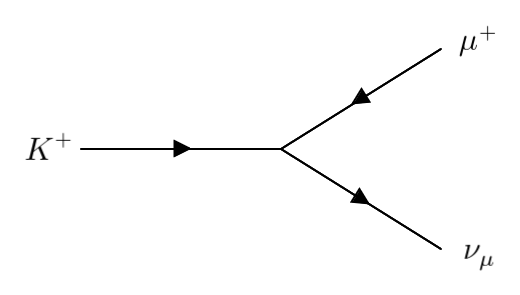
\includegraphics[width=\linewidth]{K_to_nu}
\caption{}
\end{subfigure}
\hfill
\begin{subfigure}[h]{0.4\linewidth}
\centering    
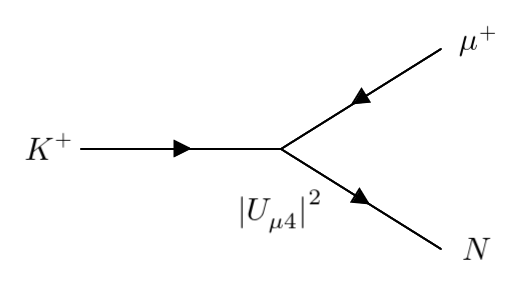
\includegraphics[width=\linewidth]{K_to_HNL}
\caption{}
\end{subfigure}%
%\hfill
\caption[kaonDiagram]{
Diagrams of the production of a SM neutrino (a) and the production of a HNL mediated by $|U_{\mu4}|^{2}$ (b) from a two-body decay of a charged kaon.
}\label{fig:kaonDiagram}
\end{figure}

%HNL from BNB beam
In general, the branching ratio $Br(\text{m}^{+}\rightarrow l^{+}_{\alpha}N)$ of a two-body decay of a charged meson $\text{m}^{+}$ into a lepton $l^{+}_{\alpha}$ ($\alpha=e,\mu,\tau$) and a HNL $N$ can be expressed in terms of the analogous branching ratio into a SM neutrino as follows \cite{HNLKelly}

\begin{equation}
	Br(\text{m}^{+}\rightarrow l^{+}_{\alpha}N) = Br(\text{m}^{+}\rightarrow l^{+}_{\alpha}\nu_{\alpha})\left(\frac{|U_{\alpha 4}|^{2}}{1 - |U_{\alpha 4}|^{2}}\right)\rho_{N}\left(\frac{m^{2}_{l_{\alpha}}}{m^{2}_{\text{m}^{+}}}, \frac{m^{2}_{N}}{m^{2}_{\text{m}^{+}}} \right) 
\end{equation}
where $Br(\text{m}^{+}\rightarrow l^{+}_{\alpha}\nu_{\alpha})$ is the branching ratio of a charged meson into a lepton and a SM neutrino, $\rho_{N}$ is a kinematic factor accounting for the available phase space of the daughter HNL in the decay, $m_{\text{m}^{+}}$ is the mass of the charged meson, $m_{l_{\alpha}}$ is the mass of the daughter lepton and $m_{N}$ is the mass of the daughter HNL.
The complete expansion of the function $\rho_{N}$ is as follows \cite{HNLKelly}

\begin{equation}
	\rho_{N}(x,y) = \frac{(x+y-(x-y)^{2})\sqrt{1+x^{2}+y^{2}-2(x+y+xy)}}{x(1-x)^{2}}
\label{eq:KinematicsFactor}
\end{equation}

%TODO: Remove s in kinematic
\begin{figure}[t] 
\centering    
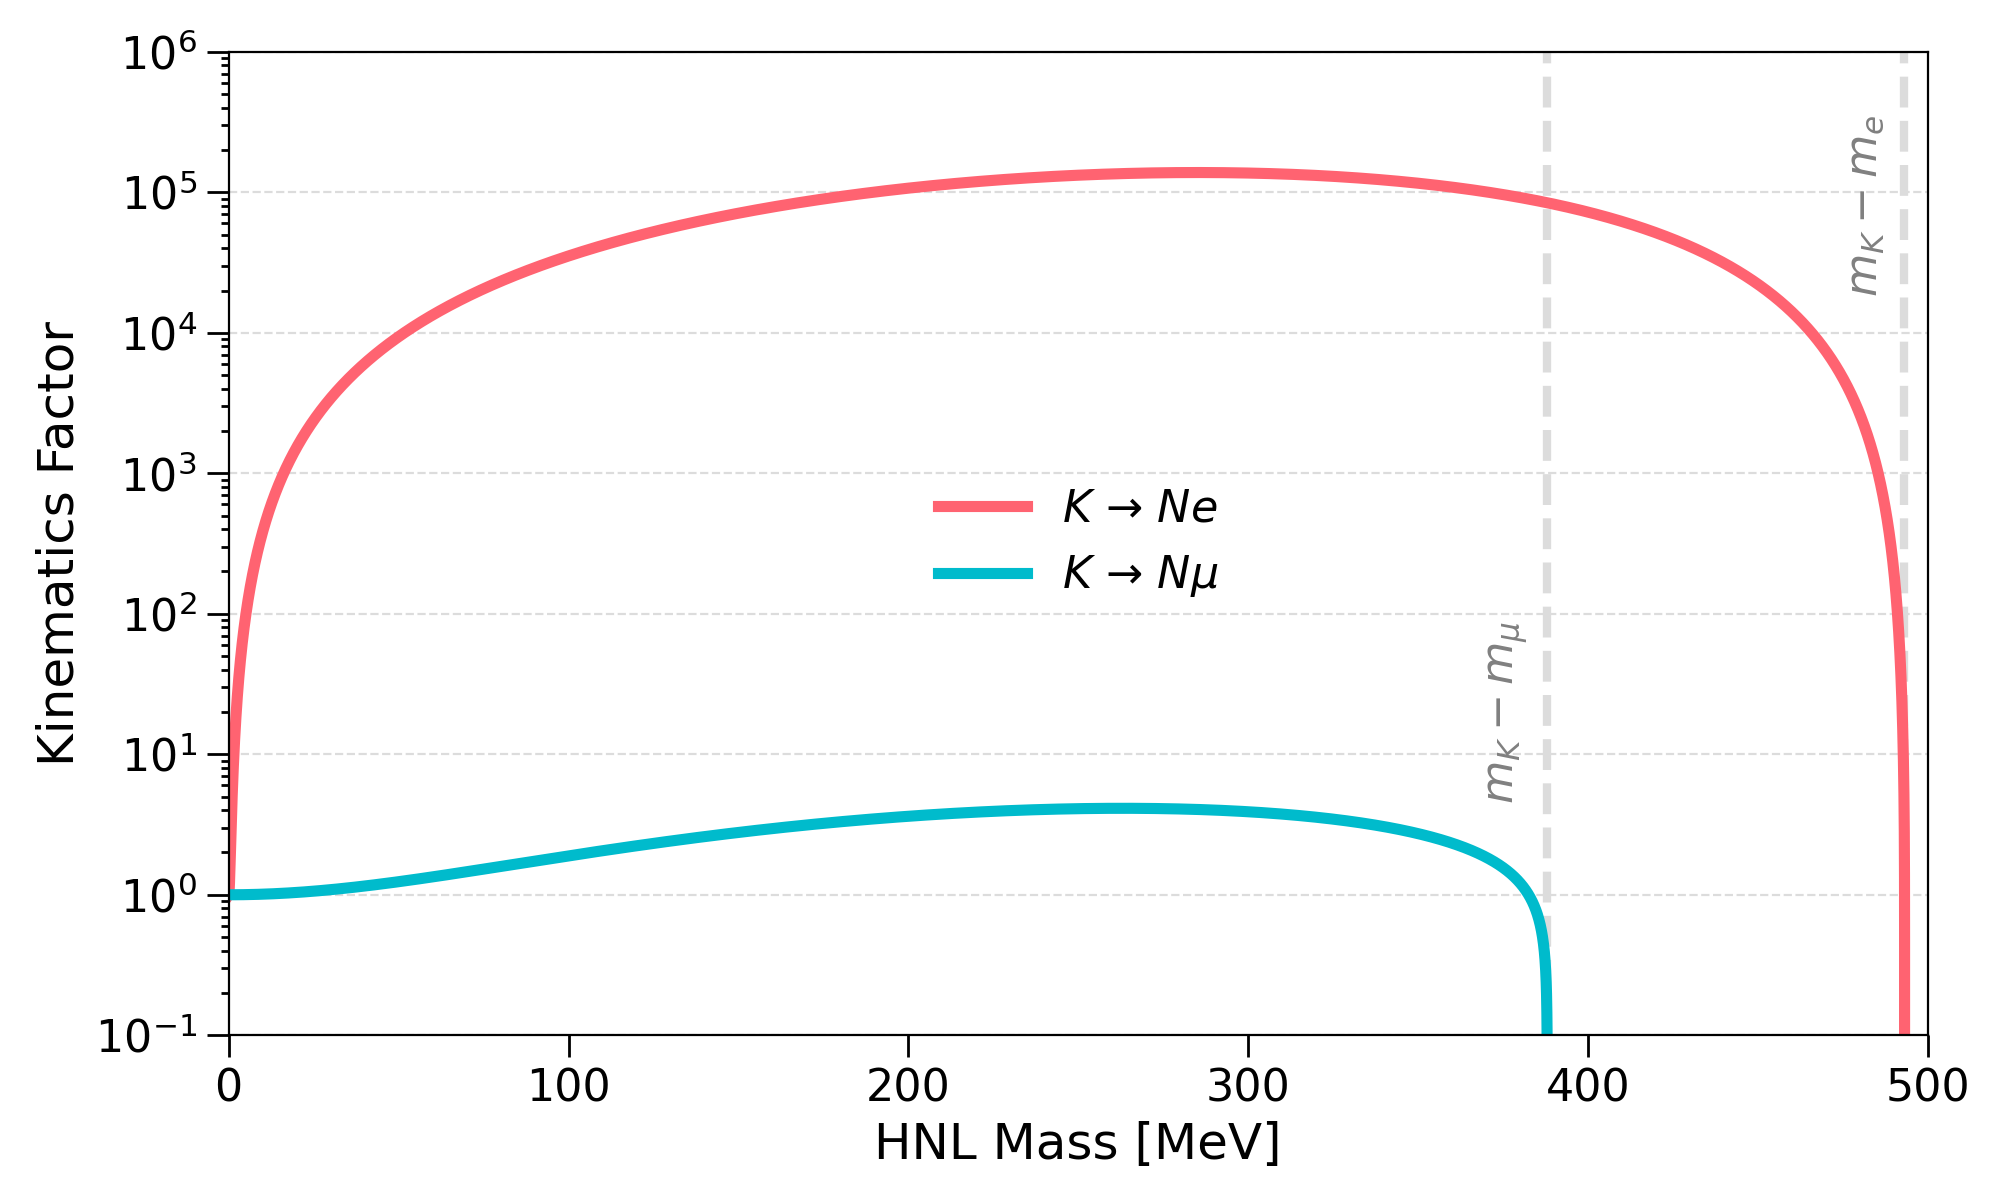
\includegraphics[width=1.0\textwidth]{kinematics_factor}
\caption[KinematicsFactor]{
The kinematic factor of HNL production rate from meson decays compared to analogous SM neutrino production, given by function $\rho_{N}$ from Eq. \ref{eq:KinematicsFactor}.
Dashed lines depict the enhancement associated with production from mesons via the mixing angle $|U_{e4}|^{2}$, whilst solid lines depict the enhancement associated with the mixing angle $|U_{\mu4}|^{2}$.
The vertical dashed grey lines indicate the mass limit on HNLs from each mixing angle.
Highlighted in pink with a thicker line width is the main production channel of HNLs studied in this thesis.
}
\label{fig:KinematicsFactor}
\end{figure}

The available phase space of HNLs is constrained by the mass of the parent meson.
Given the smaller masses of both a charged pion ($m_{\pi} = 140 $ MeV) and a charged kaon ($m_{K} = 494 $ MeV) compared to a tau ($m_{\tau}=1777 $ MeV), taus cannot be produced from meson decays in the BNB.
Consequently, only electrons and muons are produced, limiting the flavours in the mixing angle $|U_{\alpha4}|^{2}$ to $\alpha = e, \mu$.
The upper limit of the probable mass of a HNL from a two-body decay of a meson can thus be expressed as $m_{N} = m_{\text{m}^{+}} - m_{l_{\alpha}}$ ($\alpha=e,\mu$).

%Helicity Unsuppression i.e. K ->Ne and K->Nmu
%Enahancement factor??
Furthermore, the helicity suppression observed in mesons decaying into a SM neutrino has minimal effect in the same case of HNLs due to their significant mass \cite{HNLKelly}.
The contribution from helicity suppression in HNL production can be greater than one compared to neutrino production, signifying a helicity \textit{enhancement} instead.
The kinematic factor $\rho_{N}$ from Eq. \ref{eq:KinematicsFactor}, which also accounts for this enhancement, is plotted against the mass of HNLs in Fig. \ref{fig:KinematicsFactor}.
Significant enhancement is evident in the mixing angle $|U_{e4}|^{2}$, where the rate of $K^{+}\rightarrow e^{+}N$ is enhanced by a factor of $10^{5}$ and the rate of $\pi^{+}\rightarrow e^{+}N$ is enhanced by a factor of $10^{4}$.
Regarding the mixing angle $|U_{\mu4}|^{2}$, the kinematic factor for the $K^{+}\rightarrow \mu^{+}N$ channel varies between 1.5 and 4, while staying flat at 1 for the $\pi^{+}\rightarrow \mu^{+}N$ channel.

\section{Decay}
\label{sec2Decay}

%DIF with coupling
HNLs are unstable particles and therefore decay in flight with a lifetime proportional to the mixing angle $|U_{\alpha4}|^{2}$ $(\alpha=e,\mu,\tau)$, such that HNLs must survive long enough to reach the detector before decaying into SM observable particles.
Since $|U_{\alpha4}|^{2}$ is the same coupling responsible for the HNL production, the observed event rate at the detector scales with $|U_{\alpha4}|^{4}$.
At the mass $\mathcal{O}$(100 MeV), the tau-flavour mixing angle is kinematically forbidden and thus, the possible decay channels for HNLs are \cite{SBNHNL}

%Possible decay channel
\begin{equation}
\begin{split}
	N\rightarrow e^{-}\pi^{+},\qquad 
	N\rightarrow \mu^{-}\pi^{+},\qquad
	N\rightarrow \nu \pi^{0},\qquad 
	N\rightarrow \nu \gamma,\qquad \\ 
	N\rightarrow \nu e^{-} e^{+},\qquad 
	N\rightarrow \nu \mu^{-} \mu^{+},\qquad 
	N\rightarrow \nu \mu^{-}e^{+},\qquad
	N\rightarrow \nu \nu \nu. 
\end{split}
\end{equation}
In the case of HNLs are Majorana particles, the charge conjugates for the decays are also available.

\begin{figure}[t] 
\centering    
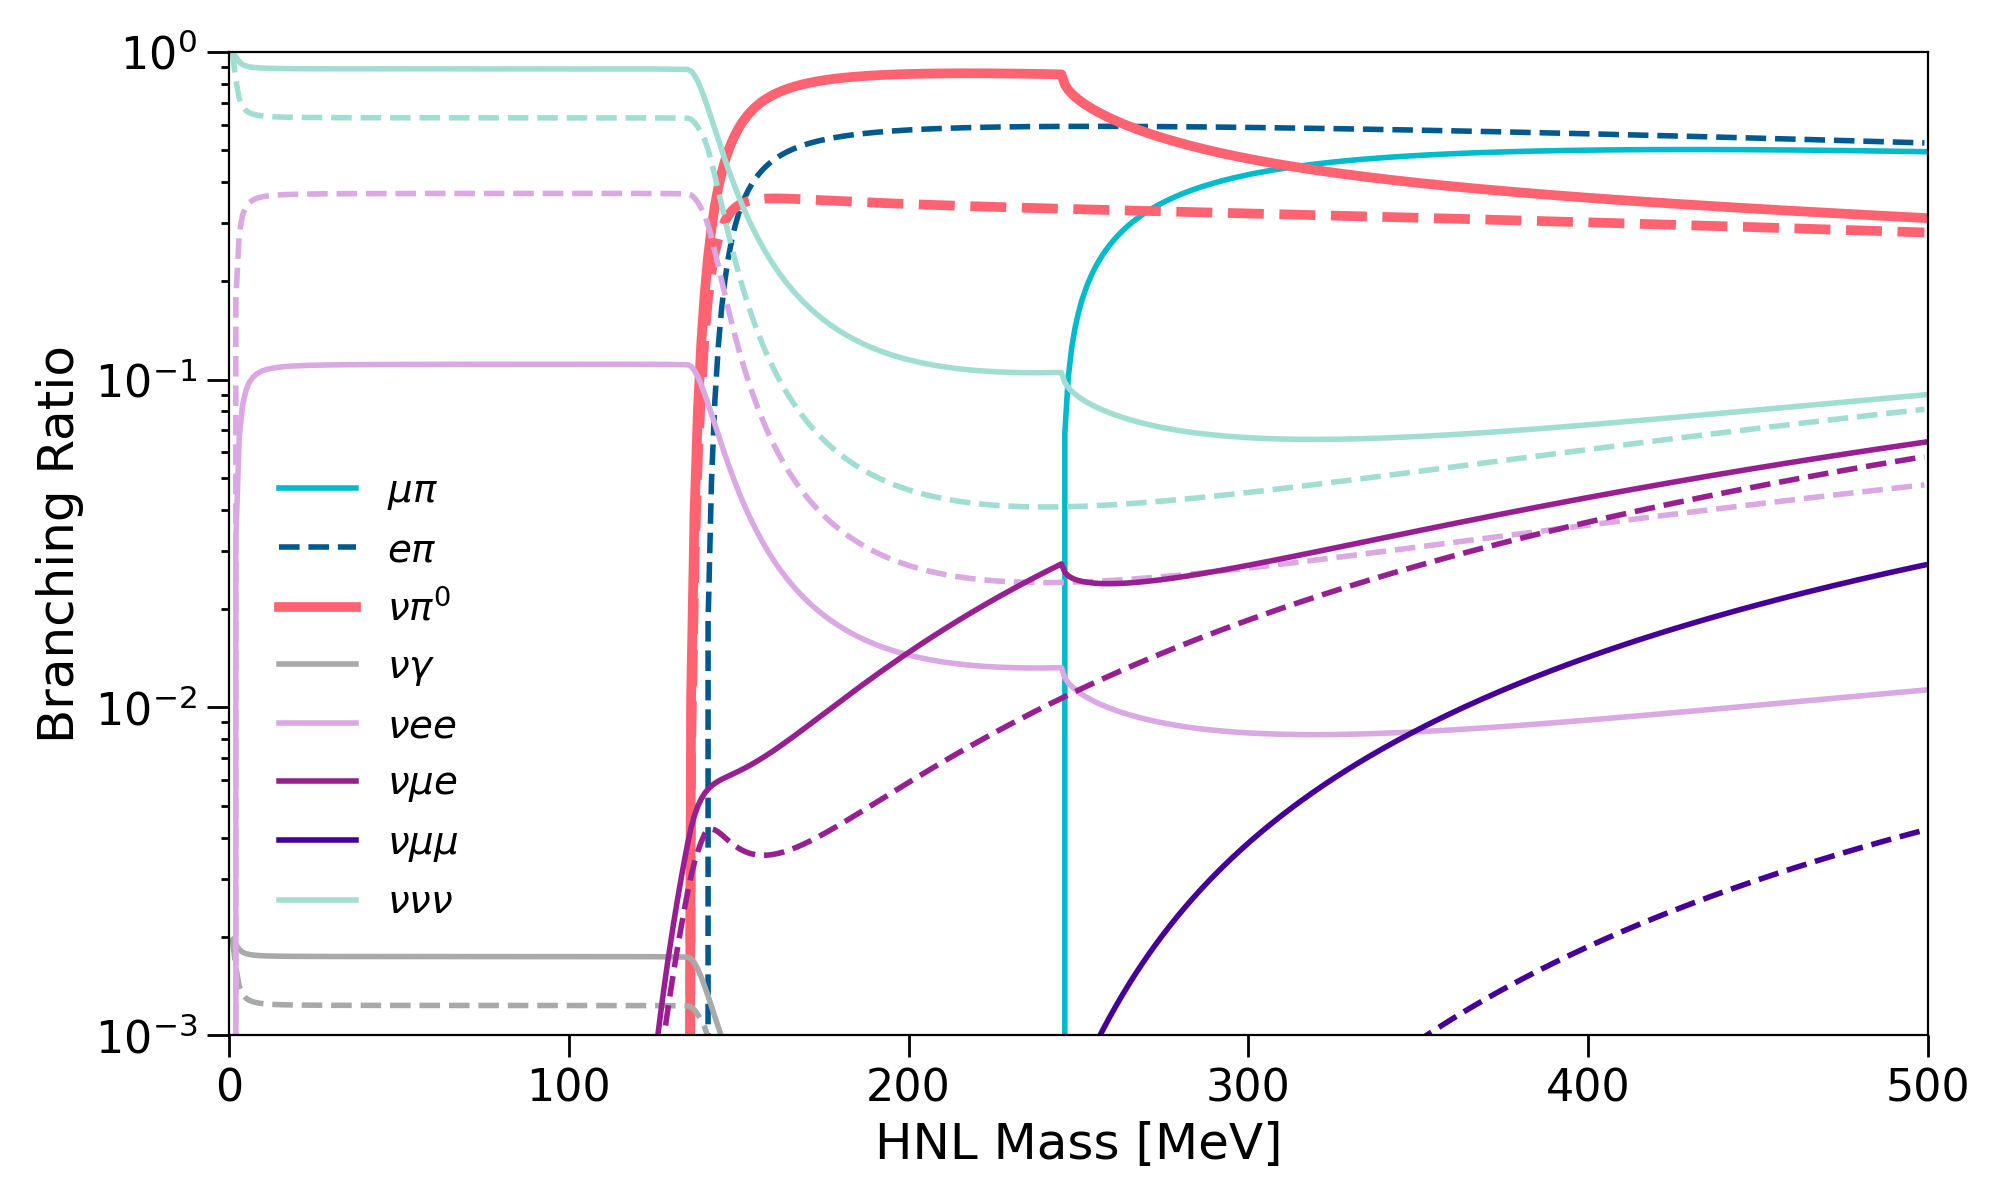
\includegraphics[width=1.0\textwidth]{branching_ratio}
\caption[branchingRatio]
{
The branching ratio of decay channels of a Majorana HNL as a function of its mass.
The decay widths are taken from Ref. \cite{HNLBin, SBNHNL, HNLZarko}.
Solid lines are branching ratios via the muon-flavour mixing angle ($[U_{e4}:U_{\mu4}:U_{\tau4}]=[0:1:0]$) and dashed lines are branching ratios via the electron-flavour mixing angle ($[U_{e4}:U_{\mu4}:U_{\tau4}]=[1:0:0]$).
Highlighted in pink with a thicker line width is the decay channel studied in this thesis: $N\rightarrow \nu \pi^{0}.$
}
\label{fig:branchingRatio}
\end{figure}

%Overall description of each BR channel
The branching ratio of decay channels for a Majorana HNL is depicted in Fig. \ref{fig:branchingRatio}, referencing decay widths from \cite {HNLBin, SBNHNL, HNLZarko}\footnote{Decay widths of HNLs have been derived independently across various literature sources. An overview of discrepancies can be found in Ref. \cite{HNLZarko}. The literature used in this thesis have been found to be in good agreement with each other.}.
For $m_{N} < 135$ MeV, the dominant branching ratio occurs in the channel $N\rightarrow \nu\nu\nu$, however this is experimentally unobservable.
Since the channel $N\rightarrow \nu \gamma$ is highly suppressed, the channel $N\rightarrow \nu e^{-}e^{+}$ provides the best sensitivity within this mass range.
In the mass range of $m_{N} > 140$ MeV for the electron-flavour mixing angle, such that a HNL has sufficient mass to decay into either a neutral pion ($m_{\pi^{0}}=135$ MeV) or a charged pion ($m_{\pi^{+}}=140$ MeV), the channel $N\rightarrow e^{-}\pi^{+}$ dominates over the channel $N\rightarrow \nu \pi^{0}$.
In the case of the muon-flavour mixing angle, the leading channel is $N\rightarrow \nu \pi^{0}$ within the mass range of $135 < m_{N} < 245 $ MeV.
Beyond $m_{N} > 245$ MeV, equivalent to the mass of a muon and a charged pion, the primary decay shifts to $N\rightarrow \mu^{-}\pi^{+}$ channel. 
Lastly, both channels $N\rightarrow \nu \mu^{-}e^{+}$ and $N\rightarrow \nu \mu^{-}\mu^{+}$ are not competitive compared to all other channels at the same mass value.  

%Desciption on the specific decay channel of thesis: HNL -> nu + pi0
This thesis searches for the existence of HNL through the decay channel $N\rightarrow\nu \pi^{0}$, which is the leading channel of the mixing angle $|U_{\mu4}|^{2}$ within the mass range of $ 135 < m_{N} < 245 $ MeV.
Sensitivity in the same mass range of the mixing angle $|U_{e4}|^{2}$ has been extensively explored.
This prompts a focus in this thesis on non-zero $|U_{\mu4}|^{2}$, assuming $|U_{e4}|^{2} = |U_{\tau4}|^{2} = 0$.  
In this mass range, the primary mode of HNL production comes from  the decay of charged kaon, due to the kinematic constrains (See Sec. \ref{sec2Production}). 

The decay width for the $N\rightarrow\nu \pi^{0}$ channel is modelled as follows \cite{HNLZarko}

\begin{equation}
	\Gamma(N\rightarrow \nu \pi^{0}) = \frac{G_{F}^{2}m_{N}^{3}}{32\pi}f^{2}_{\pi^{0}}|U_{\mu4}|^{2}\left(1-\left(\frac{m_{\pi^{0}}}{m_{N}}\right)^{2}\right)^{2}
\label{eq:pi0}
\end{equation}
where $G_{F}$ is the Fermi constant, $f_{\pi^{0}}$ is the decay constant of a neutral pion and $m_{\pi^{0}}$ is the mass of a neutral pion.
Eq. \ref{eq:pi0} taken from Ref. \cite{HNLZarko} does not contain an additional factor of 2 in the denominator as compared to Ref. \cite{SBNHNL} and \cite{HNLBin}.
The resulting event rate still agrees to the same order of magnitude.

\begin{figure}[htbp!]
%\hfill
\begin{subfigure}[h]{0.49\linewidth}
\centering    
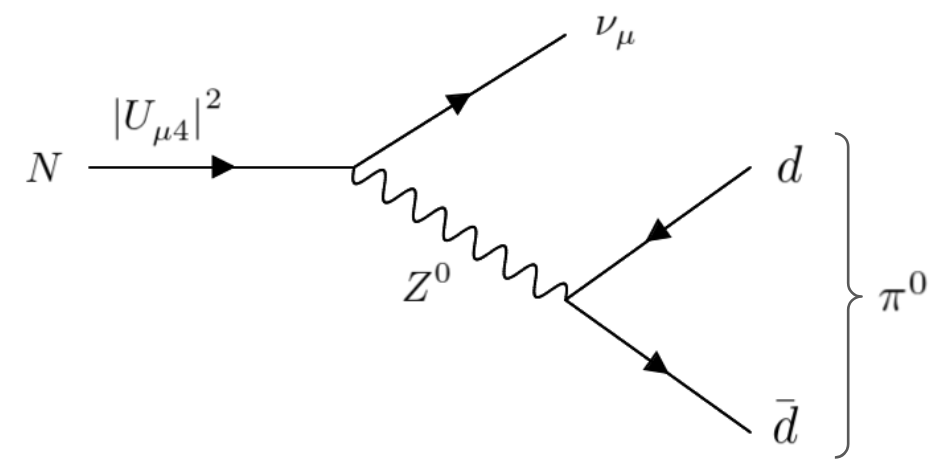
\includegraphics[width=\linewidth]{N_to_pi0_edit}
\caption{}
\end{subfigure}
\hfill
\begin{subfigure}[h]{0.49\linewidth}
\centering    
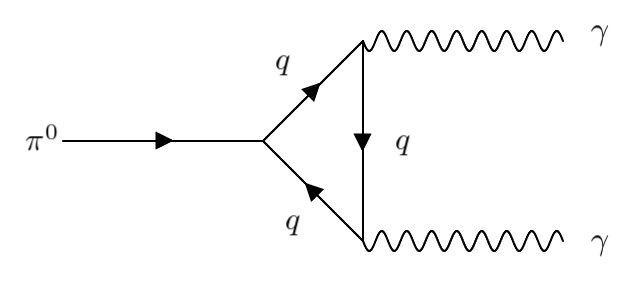
\includegraphics[width=\linewidth]{pi0_to_gam}
\caption{}
\end{subfigure}%
%\hfill
\caption[decayDiagram]{
Diagrams of a HNL decaying into a neutrino and a neutral pion mediated by $|U_{\mu4}|^{2}$ (a) and a neutral pion decaying into two photons (b).
}\label{fig:decayDiagram}
\end{figure}

%Decay signature in TPC
When a HNL decays into a neutrino and a neutral pion inside a detector, the neutrino escapes the detector undetected.
Meanwhile the neutral pion decays into two photons, with a branching ratio of 0.988 \cite{pi0}. 
Diagrams of the decays are shown in Fig. \ref{fig:decayDiagram}.
This decay results into a signature event topology inside a Liquid Argon Time Projection Chamber (LArTPC): two photon showers originating from the same vertex without any associated hadronic activities.
Neutral-current neutrino interactions that result in a neutral pion also share the same final state particles and thus, constituting the main background for this search.
Nonetheless, differences in event kinematics and precise timing resolution, as detailed in Sec. \ref{}, enable an effective separation between HNL signals and the neutrino backgrounds. 

%Dirac or Majorana Nature
As discussed in Sec. \ref{sec2Overview}, HNLs can be either Dirac or Majorana particles in nature.
Majorana HNLs violate the conservation of lepton numbers, whereas Dirac HNLs preserve it.
Consequently, the expected event rate of Majorana HNLs is double that of Dirac HNLs.
Moreover, the helicity of decay products differs between Majorana and Dirac HNLs.
Majorana HNLs decay isotropically, whereas in the case of Dirac HNLs, the helicity of the daughter neutrino determines the direction of the other daughter particles in the same decay \cite{HNLSilvia}.
A HNL decaying into a neutrino and a neutral meson is isotropic in the rest frame, and thus, this channel is insensitive to the Dirac nature of HNLs.
As a result, this thesis assumes HNLs are Majorana particles.

\section{Previous Experimental Searches}
\label{sec2Previous}

%Number of fermion families = Z boson decay for LH neutrinos, RH neutrinos is not constrained

%Overview of different types of searches
HNLs have been searched by experiments over the decades, across a wide range of mass.
Oscillation experiments and precise $\beta$ decay experiments have probed HNLs in the mass range between eV and keV, while collider experiments have primarily explored GeV-scale HNLs.
To date, no evidence of HNL existence has been found, and thus, experiments have set upper limits on the coupling $|U_{\alpha4}|^{2}$ $(\alpha=e,\mu,\tau)$.
The sensitivity contour of HNL is commonly expressed in terms of the mixing angle $|U_{\alpha4}|^{2}$ as a function of the HNL mass.

Here, current experimental limits on HNLs around $\mathcal{O}$ (100 MeV) are presented, focusing specifically on the mass range of $ 0 < m_{N} < 245 $ MeV, which is relevant to the final states $\nu\pi^{0}$.
The summary is plotted in Fig. \ref{fig:Sensitivity}.
In this mass range, two key experimental methods are peak searches and decay searches.
Peak searches probe only the production rate of HNLs, whereas decay searches probe both production and decay rates.


\subsection{Peak Searches}

Peak search experiments measure the energy spectrum  resulting from the decay of meson decay that would produce a HNL. 
Typically, the two-body leptonic decay of a meson is modelled as $\text{m}\rightarrow l + Missing$, where $\text{m}$ is the parent meson (a pion or a kaon) and $l$ is the daughter particle (a pion or a lepton) \cite{OwenPhD}.
The \textit{missing} decay products are attributed to either HNLs or SM neutrinos.
HNLs are expected to exit the detector before decaying, whereas SM neutrinos escape the detector before interacting, serving as the primary background for this search.
Since the momenta of m and $l$ are precisely measured, the missing invariant mass can therefore be derived as $m^{2}_{miss} = (P_{\text{m}} - P_{l})^{2}$, where $P_{\text{m}}$ and $P_{l}$ are the 4-momentum of the parent and daughter particles.
Given the near-zero mass of SM neutrinos, the mass of the daughter HNL can be treated as $m_{N} = m_{miss}$.
Consequently, an excess over the background at $m_{miss}$ would indicate potential existence of HNLs.

To infer the sensitivity contour, the flavour of the daughter lepton determines the flavour of the mixing angle, while the amplitude of the decay spectrum at $m_{miss}$ determines its upper limit.
Limits placed by the peak searches are insensitive to the Dirac or Majorana nature of HNLs as it does not impact the kinematics of the meson decay.
For the mixing angle $|U_{\mu4}|^{2}$, the most competitive limits have been established by the following experiments, particularly on pion and kaon decay spectrum.

\subsubsection{Pion Decay Spectrum Peak Searches}

\begin{coloritemize}
\item \textbf{SIN} (Swiss Institute for Nuclear Research) performed a peak search using stopped positive pions decay via the channel $\pi^{+} \rightarrow \mu^{+} + Missing$, using a scintillator in 1981 and a germanium detector in 1987.
The pion enabled probing HNLs within the low mass range of $\mathcal{O}$(10 MeV).
Upper limits of $|U_{\mu4}|^{2}$ were placed in the mass range 1--20 MeV at $10^{-4}$ \cite{SIN1, SIN2, SIN3}.

\item The \textbf{PIENU} collaboration at TRIUMF also searched for HNLs using stopped pions.
The most recent result in 2019 set the most stringent limits on $|U_{\mu4}|^{2}$ in the range $10^{-5}$ in the mass range of 15--34 MeV \cite{PIENU}, extending beyond result reported by SIN.

\end{coloritemize}

\subsubsection{Kaon Decay Spectrum Peak Searches}

\begin{coloritemize}
\item The \textbf{KEK} collaboration conducted an experiment known as E89, which aimed to search for HNLs using the muon range spectrum resulting from stopped kaon decays during 1981--1982. 
Following this, experiment E104 in 1983 was carried out with improved momentum resolution and background suppression.
The kaons were produced using a 0.5 GeV proton beam, and $3 \times 10^{6}$ muons from kaon decays were analysed using magnetic spectrograph.
The outcomes from the E89 experiment constrained the limits of $|U_{\mu4}|^{2}$ between 10$^{-4}$--10$^{-6}$ within the mass range of 70--300 MeV.
Additionally, the combined results from the E89 and E104 experiments extended the sensitivity towards the lower mass range between 45--300 MeV, although these findings are currently unpublished \cite{KEK1, KEK2, KEK3}.

\item The \textbf{E949} collaboration at Brookhaven National Laboratory performed a kaon decay experiment using 21.5 GeV protons in 2002.
The analysis on the decays of $2 \times 10^{21}$ stopped kaons resulted in limits on $|U_{\mu4}|^{2}$  within the mass range between 175--300 MeV, constraining at 10$^{-7}$--10$^{-9}$ \cite{E949}.

\item The \textbf{NA62} collaboration, a kaon decay experiment at the CERN super proton synchrotron, analysed $10^{8}$ stopped kaons from 400 GeV protons extracted from the synchrotron.
The first results from a data set in 2015 set upper limits on $|U_{\mu4}|^{2}$ in the range of 10$^{-7}$--10$^{-6}$ for HNL masses in the range 250--373 MeV.
Updated results using a larger dataset collected in 2016--2018 significantly improved the limits by an order of magnitude to 10$^{-8}$--10$^{-7}$, and extended the mass range to 200--384 MeV \cite{NA62A, NA62B}.
\end{coloritemize}

\subsection{Decay Searches}

Decay searches look for decay products from HNLs.
HNLs are typically produced outside of the detector before reaching it, potentially decaying into SM observables inside the detector.
Different combinations of production and decay channels yield different expected event rates, allowing for exploring different sensitivity regions associated with different mixing angles.
Decay searches have been historically performed in beam-dump experiments, designed explicitly to suppress background from SM interactions, thereby enabling the search for rare decay processes.
Recently, modern neutrino oscillation experiments with enhanced resolution have emerged as competitive beam-dump experiments alongside their neutrino physics programme.
For $|U_{\mu4}|^{2}$ within the mass range of 0--245 MeV, the most competitive limits have been set by the following experiments.

\begin{coloritemize}
\item The CERN \textbf{PS191} experiment in 1984 utilised an exposure of 19.2 GeV protons on a beryllium target, generating $10^{19}$ Proton On Target (POT).
The detector was positioned at 128 m from the target at an off-axis angle of $2.3^{\circ}$ with respect to the beam direction.
It was designed specifically to search for HNLs by maximising the signal rate while minimising the background rate.
The 216 m$^{3}$ volume (12 m long and a cross-sectional area of 18 m$^{2}$) was filled with helium.
The sparse medium was chosen to reduce background rates arising from SM neutrino interactions, leveraging the large volume to provide a high rate of HNL signals. 
Limits on $|U_{\mu4}|^{2}$ within the mass range of 120--350 MeV were placed in the range of 10$^{-5}$--10$^{-9}$ \cite{PS191A, PS191B}.
A re-evaluation in 2022 found the limits to be lower than the original published results \cite{PS191C}.
	
%\item The \textbf{T2K} collaboration recently searched for HNLs using the near detector ND280, located 280 m from the beam target at an off-axis angle of $2.04^{\circ}$.
%The analysis was performed on the data collected from 2010-2017, with a beam intensity of 30 GeV proton on graphite target and an exposure of $\approx 2 \times 10^{21}$ POT.
%The search was limited to the three argon gas TPC volumes, which minimised the neutrino background rate due to the low gas density.
%The results constrained the limits of $|U_{\mu4}|^{2}$ in the range of 10$^{-8}$--10$^{-9}$ for the HNL mass between 250--380 MeV \cite{T2KHNL}.
%The T2K collaboration has also presented results on $|U_{\mu4}|$ in the case where $|U_{e4}|$ and $|U_{\tau4}|$ are assumed to be non-zero and marginalised using results from other channels.

\item The \textbf{NuTeV} collaboration at Fermilab conducted HNLs searches in 1996 using a high energy neutrino beam produced by protons accelerated from the Tevatron ring.
The dataset comprised of an exposure of $3 \times 10^{18}$ POT with an energy of 800 GeV.
HNLs were produced from the $D$ mesons resulting from proton collisions with the target.
This enabled exploration of HNL masses up to 2000 MeV, surpassing any other beam-dump experiments described here.
The experiment established limits on $|U_{\mu4}|^{2}$ in the range 10$^{-6}$--10$^{-7}$ within the mass range of 225--2000 MeV \cite{NuTeV}.

\item The \textbf{MicroBooNE} collaboration conducted a series of searches for HNLs using a LArTPC, beginning with the first result in 2020 and subsequent results in 2022 and 2023.
The initial analysis was performed using an exposure of $2 \times 10^{20}$ POT obtained from the on-axis BNB.
A special delayed trigger was implemented to identify HNLs arriving at the detector later than SM neutrinos.
Limits on $|U_{\mu4}|^{2}$ were set in the range of $10^{-7}$ for HNL masses spanning between 260--385 MeV.
The latter two searches focused on HNLs arising from kaons decays in the NuMI absorber, which arrived at the detector at an angle to SM neutrinos from the BNB.
The dataset comprised of two runs with an exposure of $2 \times 10^{20}$ and $5.01 \times 10^{20}$ POT.
The combined results incorporated multiple HNL decay channels, probing a wide mass spectrum between 10--385 MeV.
Notably, these recent results have set the most stringent limits to date on $|U_{\mu4}|^{2}$, ranging between in the range 10$^{-4}$--10$^{-7}$ within the mass range of 34--175 MeV, thus extending the findings from 2019 \cite{uboone1, uboone2, uboone3}.

\end{coloritemize}

\begin{figure}[t] 
\centering    
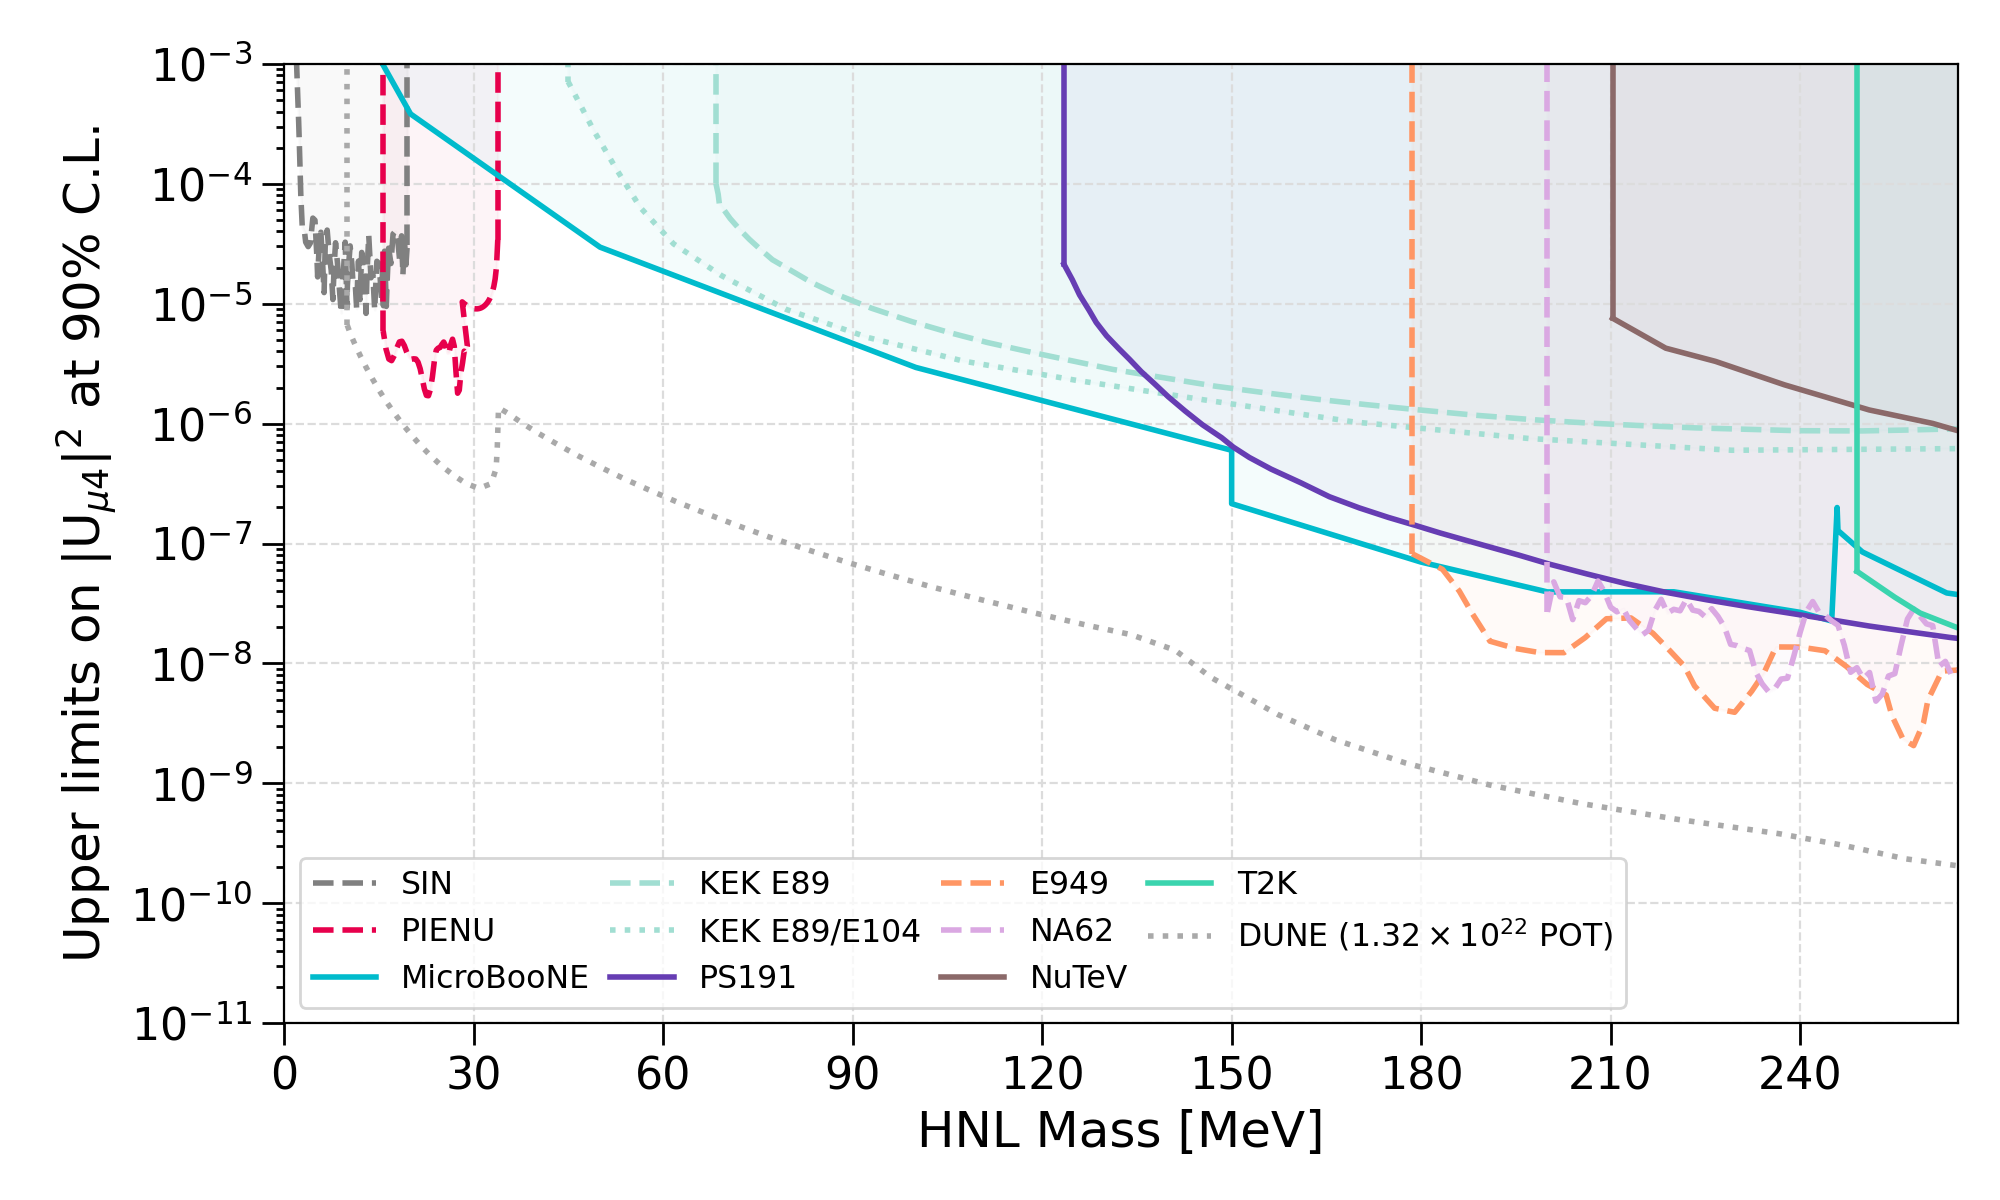
\includegraphics[width=1.0\textwidth]{sensitivity}
\caption[Sensitivity]{
Sensitivity contour of the upper limits on the mixing angle $|U_{\mu4}|^{2}$ for Majorana HNLs, within the mass range of $0 < m_{N} < 245$ MeV.
Dashed lines show the constraints derived from peak searches, whilst solid lines show the limits set by decay searches.
The dotted line shows the unpublished limit from the KEK E89/E104 experiments.
}
\label{fig:Sensitivity}
\end{figure}


%TODO: Add concluding remarks
\section{Concluding Remarks}

HNLs are BSM particles that provide a natural explanation not just for the mass generation of active neutrinos but also for their extreme lightness.
The SBND, located only 110 m from the BNB, is capable of detecting HNLs coming from meson decays in the beam, which then decay in flight inside the detector.
Novel light detection and reconstruction techniques, resulting in precise timing resolution, enables the separation of HNL signals from SM neutrino backgrounds (See Chapter \ref{}).
Here, the focus is on the $\nu\pi^{0}$ final state, distinctive event topology featuring two forward-going photon showers without any hadronic activities at the shared vertex.
In the mass range between $135 < m_{N} < 245$ MeV of the mixing angle $|U_{\mu4}|^{2}$, the sensitivity is relatively unexplored.
This presents a compelling opportunity for SBND to set competitive limits in this region.
